\section{Systemmodelle}
\subsection{Backend}
\begin{figure}[htbp]
	\centering
	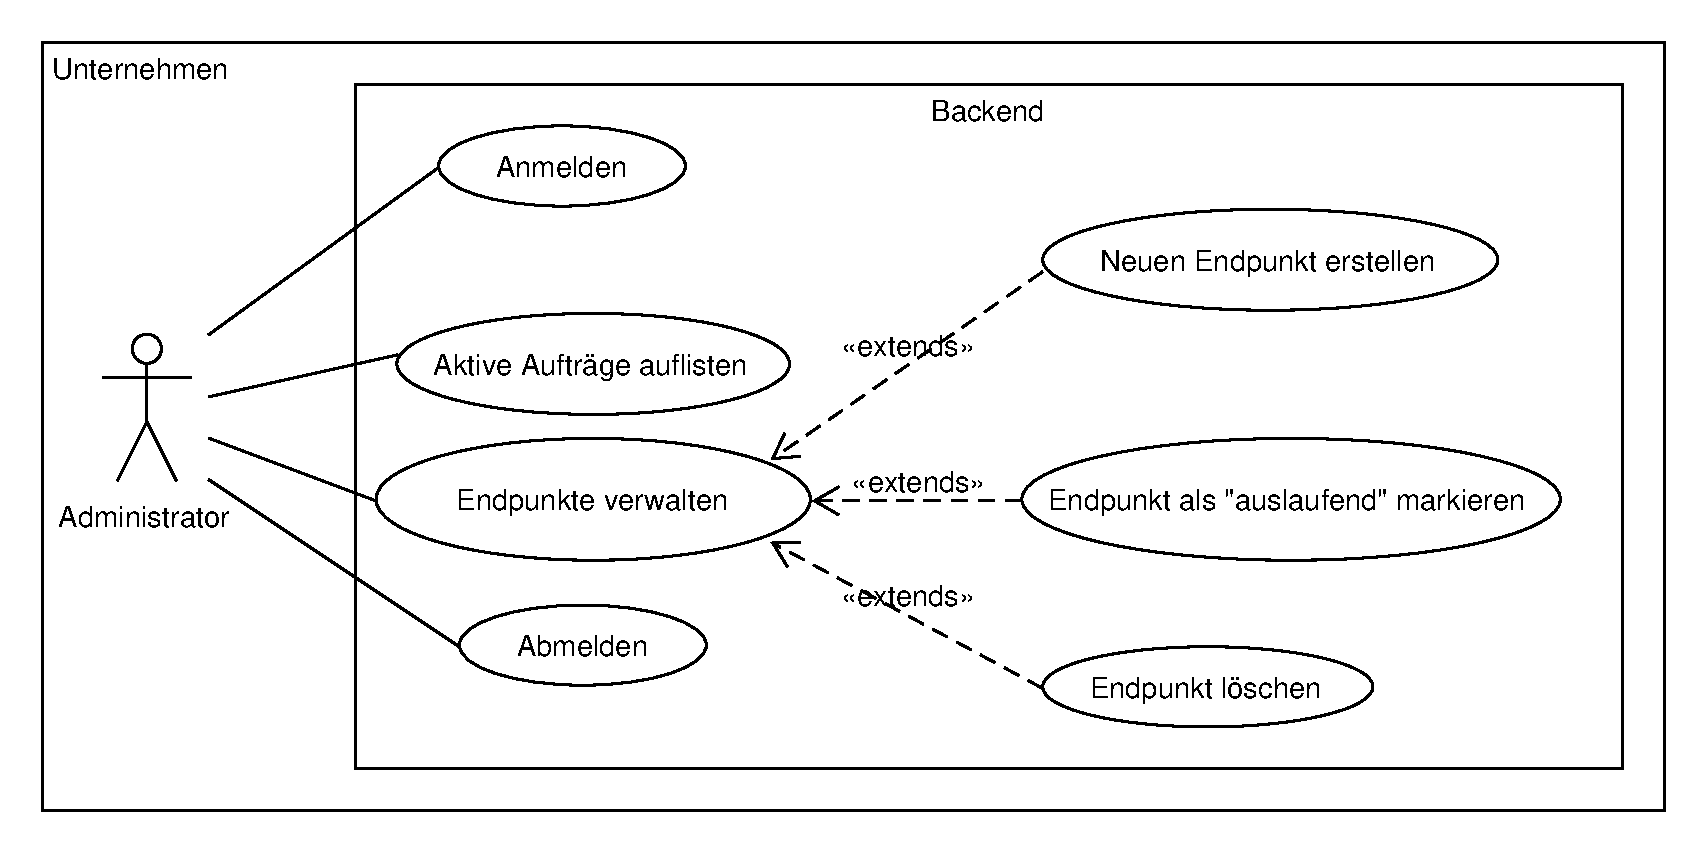
\includegraphics[width=1.0\textwidth]{UseCase_Admin.pdf}
	\caption{Aktionsübersicht des Administrators}
	\label{fig:Bild1}
\end{figure}
\subsubsection{Szenario: Endpunktkonfiguration}
\paragraph{Beschreibung}
Der \gls{Administrator} nimmt die Konfiguration eines neuen \glslink{Endpunkt}{Endpunkts} im bestehenden \gls{System} vor.
Der neue Endpunkt stellt einen neuen Kontext dar, um das Mehr-Augen-Prinzip effizient umzusetzen.
Nach erfolgreicher Konfiguration können die \gls{Nutzer} den Endpunkt nutzen, um einen \gls{Auftrag} in diesem Kontext zu stellen.

\paragraph{Korrekter Ablauf}
Der Administrator hat sich im System angemeldet und befindet sich in der Administratoren-Übersicht des \glslink{Backend}{Backends}.
Er klickt auf den \enquote{Endpunkt erstellen}-Button und wird zu einem \gls{Editor} weitergeleitet.
Dort wählt er den Namen \enquote{Urlaubsantrag} für diesen Endpunkt.
Im Editor findet er eine Vielzahl an Konfigurationselementen. Ein Großteil davon liegt in der Form von Schaltern vor, die Kriterien ein- oder ausschalten. Zu diesen gehören die Benachrichtigung für Auftragserhaltende, die Löschbarkeit eines Auftrags durch den Auftragsersteller, die Art der \gls{Signatur} und ob ein Nutzer weitere Augenpaare hinzufügen kann.  Es besteht die Möglickeit ein \gls{Formular} zu definieren, das vom Auftragsersteller ausgefüllt werden muss. Andere Konfigurationselemente dienen dem Hinzufügen, Entfernen und Spezifizieren der benötigten Signaturen.
Der Administrator konfiguriert den Endpunkt wie folgt:
\begin{itemize}
	\item Anzahl der Augenpaare: vier
	\item sequentieller \glslink{Modus}{Signaturmodus}
	\item \gls{LDAP}-\glspl{Rolle} in entsprechender Reihenfolge: Sekretariat, Personalleitung, Chef
	\item E-Mail-Benachrichtigungen für Auftragserhaltende sind deaktiviert.
	\item Eine Signatur wird durch Klicken eines Bestätigungsbuttons erfüllt.
	\item Ein Auftrag, der abgelehnt wurde, kann vom Auftragssteller gelöscht werden.
	\item Der Auftragssteller erhält eine Benachrichtigung, wenn sein Auftrag genehmigt wurde.
\end{itemize}
Der Administrator bestätigt diese Konfiguration durch Klicken auf den \enquote{Erstellen}-Button.
Er wird auf die Startseite des Backends weitergeleitet.
Angemeldete Nutzer sehen einen neuen Endpunkt in der Endpunktauflistung und können diesen nutzen.

\paragraph{Abgebrochener Ablauf}
Der Administrator bricht die Endpunktkonfiguration an beliebiger Stelle durch Klicken des \enquote{Abbrechen}-Buttons ab.

\subsubsection{Szenario: Endpunkt entfernen}
\paragraph{Beschreibung}
Aufgrund einer Änderung der Firmenpolitik müssen nun alle wichtigen, die Firma betreffenden Anträge nicht mehr nur vom CEO (Chief Executive Officer), sondern auch vom CFO (Chief Financial Officer) signiert werden. Deshalb muss der bereits bestehende Endpunkt \enquote{Wichtige Anträge} entfernt werden und durch einen neuen  mit Berücksichtigung der Signatur des CFO erstellt werden.
\paragraph{Korrekter Ablauf}
Dazu klickt der bereits angemeldete Administrator in der Administratorübersicht auf den Menüpunkt \enquote{Endpunkt entfernen}. Der Administrator wird gebeten, den zu entfernenden Endpunkt auszuwählen. Er wählt den Endpunkt \enquote{Wichtige Anträge} aus und klickt auf \enquote{Endpunkt entfernen}. Dem Administrator wird der Hinweis angezeigt, dass Endpunkte erst dann entfernt werden können, wenn alle aktiven Aufträge fertiggestellt sind. Da noch immer aktive Aufträge laufen, wird der Administrator gefragt, ob er den Endpunkt als \enquote{auslaufend} markieren möchte. Er muss bestätigen, dass nun keine neuen Aufträge für diesen Endpunkt angenommen werden können. In seiner Ansicht wird nun unter dem Menüpunkt \enquote{Endpunkte verwalten} der Name des Endpunkts \enquote{Wichtige Aufträge} ausgegraut angezeigt.
Er konfiguriert den neuen Endpunkt und meldet sich vom Backend ab.
\paragraph{Abgebrochener Ablauf}
Falls der Administrator das Fenster schließt, nicht auf den \enquote{Endpunkt löschen}-Button drückt oder das Löschen nicht bestätigt, wird die Löschung des Endpunkts nicht vorgenommen.


\subsection{Frontend}
\begin{figure}[htbp]
	\centering
	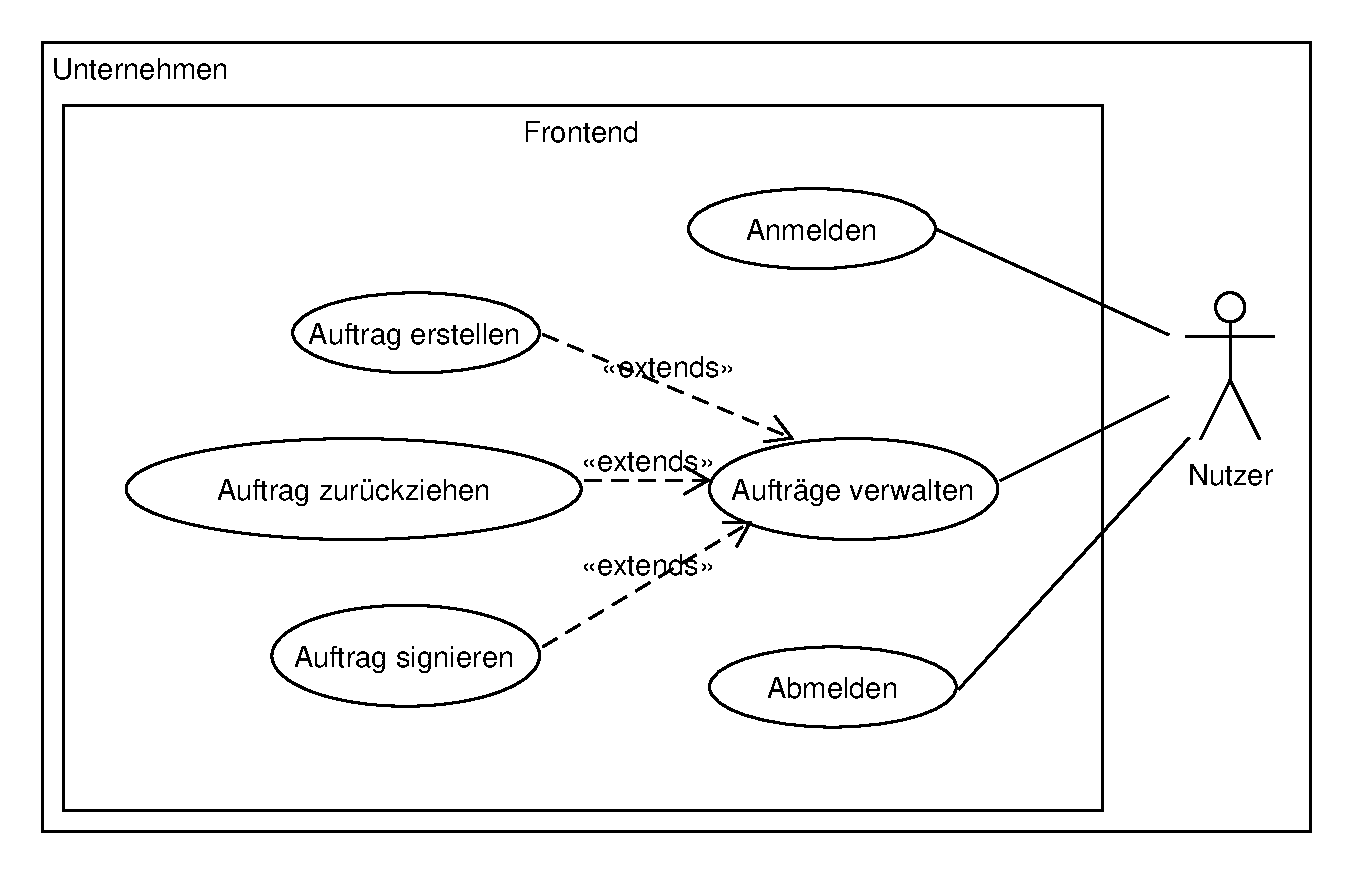
\includegraphics[width=1.0\textwidth]{UseCase_User.pdf}
	\caption{Aktionsübersicht des Nutzers}
	\label{fig:Bild2}
\end{figure}

\subsubsection{Szenario: Auftrag erstellen}
\paragraph{Beschreibung}
Nicolas möchte einen neuen Auftrag unter einem bestehenden Endpunkt für einen GUI-Entwurf einer Webseite, die Hundewelpen vermittelt, erstellen. Der GUI-Entwurf muss dafür von vier seiner Teamkollegen abgezeichnet werden.
\paragraph{Korrekter Ablauf}
Der Nutzer meldet sich am \gls{Frontend} an. Er wählt in der Auflistung der Endpunkte den Punkt \enquote{Zehn-Augen} aus. Er wird zur Erstellungsseite eines Auftrags für diesen Endpunkt weitergeleitet. Der Nutzer gibt folgende Konfiguration an:
\begin{itemize}
	\item Auftragsname: \enquote{Hundewelpen-Seite, GUI-Entwurf}.
	\item Signaturmodus: sequentiell
	\item Rollen: Wendy, Moritz, Noah, Julius (seine vier Teamkollegen)
	\item Benachrichtigung per E-Mail bei \gls{Status}änderung ist eingeschaltet.
\end{itemize}
\newpage
Er fügt den GUI-Entwurf als PDF-Datei hinzu. Dafür drückt er auf den \enquote{Datei hochladen}-Button und wählt seinen Entwurf im Dateiauswahldialog aus. Er bestätigt seine Konfiguration durch Klicken auf den \enquote{Auftrag erstellen}-Button. Nicolas wird zur Startseite des Frontends weitergeleitet und kann den erstellten Auftrag unter dem Punkt \enquote{Meine Aufträge} einsehen. Er erhält eine Bestätigungs-E-Mail mit allen Auftragsdetails.

\paragraph{Abgebrochener Ablauf}
Vor der Bestätigung durch den \enquote{Auftrag erstellen}-Button kann der Nutzer die Auftragserstellung an beliebiger Stelle abbrechen, indem er auf den \enquote{Abbrechen}-Button klickt oder das Fenster schließt.

\subsubsection{Szenario: Auftrag signieren}
\paragraph{Beschreibung}
Die Nutzer der Rolle \enquote{Personalabteilung} wurden per E-Mail benachrichtigt, dass ein neuer zu signierender Auftrag mit dem Betreff \enquote{Urlaubsantrag, Thomas Mayer} eingegangen ist. Ein Mitarbeiter der Personalabteilung kümmert sich um die Signierung des Auftrags.
\paragraph{Korrekter Ablauf}
Der Mitarbeiter der Personalabteilung meldet sich am Frontend an und wird auf die Startseite weitergeleitet. Durch Klicken auf den Menüpunkt \enquote{Zu signierende Aufträge} unter dem Reiter \enquote{Aufträge} kann er sich alle Aufträge auflisten lassen, die er mit seiner Rollen-Zugehörigkeit signieren kann. In der Auflistung der Aufträge klickt er auf den Auftrag \enquote{Urlaubsantrag, Thomas Mayer}. Er bekommt eine Detailansicht des Auftrags mit den folgenden Informationen zu sehen:
\begin{itemize}
	\item Fortschritt: noch nicht signiert
	\item Zugehörige Datei: Urlaubsantrag.pdf
	\item Anzahl der Augenpaare: vier
	\item Signaturmodus: sequentiell
	\item Signaturart: Button klicken
\end{itemize}
Der Mitarbeiter der Personalabteilung lädt sich die Datei \enquote{Urlaubsantrag.pdf} über den \enquote{Datei herunterladen}-Button herunter. Er prüft den Auftrag und signiert ihn, indem er auf den \enquote{Auftrag signieren}-Button klickt. Nach nochmaliger Bestätigung ist der Auftrag signiert.

\paragraph{Abgebrochener Ablauf}
Falls der Mitarbeiter das Fenster schließt, nicht auf den \enquote{Auftrag signieren}-Button drückt oder die Signatur des Auftrags nicht erneut bestätigt, wird die Signatur abgebrochen.
